\documentclass[12pt, letterpaper, twoside]{article}

\usepackage[utf8]{inputenc}
\usepackage{listings}
\usepackage{color}
\usepackage{algorithm}
\usepackage{algpseudocode}
\usepackage{graphicx}
\usepackage{amsmath}
\usepackage{algpseudocode}
\usepackage{enumitem}

\graphicspath{ {./images/} }

\definecolor{dkgreen}{rgb}{0,0.6,0}
\definecolor{gray}{rgb}{0.5,0.5,0.5}
\definecolor{mauve}{rgb}{0.58,0,0.82}

\lstset{frame=tb,
  language=C,
  aboveskip=2mm,
  belowskip=2mm,
  showstringspaces=false,
  columns=flexible,
  basicstyle={\small\ttfamily},
  numbers=none,
  numberstyle=\tiny\color{gray},
  keywordstyle=\color{blue},
  commentstyle=\color{dkgreen},
  stringstyle=\color{mauve},
  breaklines=true,
  breakatwhitespace=true,
  tabsize=2
}

\title{%
Design and Analysis of Algorithms\\
\large 6.3 Dynamic Programming Exercises
}
\author{Daniel Shannon}
\date{May 16th, 2022}

\begin{document}
\begin{titlepage}
\maketitle
\end{titlepage}
\section*{6.3.2}
\begin{quote}
  \begin{itemize}
    \item You have a sequence of numbers $x_1, x_2,x_3,...,x_n$
    \item Find the contguous subsequence [$x_i,...,x_j$] with the greatest sum
    \item Not allowed to skip elements!
    \item Use dynamic programming to find an $O(n)$ solution
  \end{itemize}
  
\end{quote}
\subsection*{My Answer}
\begin{center}
    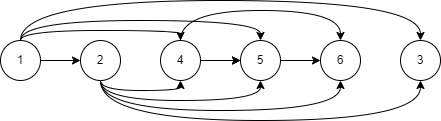
\includegraphics[scale=.6]{6_3_2.png}
    \\ example linearized DAG
\end{center}
Similar to largest increasing subsequence, but we track the sum instead of the length.
\begin{algorithmic}
  \State $prev(0)=x_1$
  \ForAll {$j=1,2,...n$, in linearized order}
  \State $sum_j$+=$max\{S[j]+x_j:(i,j)\in{E}\}$
  \If{$S[j]<sum_j$}
  \State $S[j]=sum_j$
  \State $prev(j)\cdot{(i,j)}$ concat
  \EndIf
  \EndFor
\end{algorithmic}
\subsection*{Solution}
\begin{algorithmic}
  \State $S[j]$ maximum sum of a cont subsequence ending at index $j$
  \State $S[j]=max\{A[j],S(j-1)+A[j]\}$
  \State $S[0]=0$
  \ForAll {$j=1,2,...n$, in linearized order}
  \State $S[j]=max\{A[j],S(j-1)+A[j]\}$
  \EndFor
\end{algorithmic}
\newpage
\section*{6.3.4}
\begin{quote}
  \begin{itemize}
    \item You are trying to decide where to build a chain of restaurants along a linear highway.
    \item At each location $i$ along the highway, you will make a profit of $p(i)$ that depends on the location.
    \item You are not allowed to put two restaurants within $k$ miles of each other.
    \item Where should you place the restaurants to maximize profit?
    \item Hint: Draw the DAG!
  \end{itemize}
\end{quote}
\subsection*{My Answer}
\begin{center}
  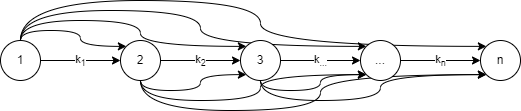
\includegraphics[scale=0.6]{6_3_4.png}
\end{center}
\begin{algorithmic}
  \State $P[j]$ max profit ending at index $j$
  \State $P[j]=max\{p_j,(i,j)\in{E}:M(i)+p\}$
  \State $P[0]=0$
  \State $dist(0)=0$
  \ForAll {$j=1,2,...n$, in linearized order}
  \State $P[j]=max\{p_j-k,(i-k,j)\in{E}:P(i-k)+p\}$
  \EndFor
\end{algorithmic}

\subsection*{Solution}
\begin{center}
  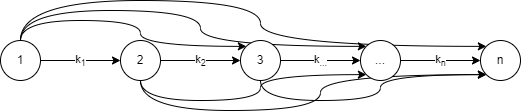
\includegraphics[scale=0.6]{6_3_4_solution.png}
\end{center}
\newpage
\section*{6.3.6}
\begin{quote}
  \begin{itemize}
    \item Suppose you have two strings of length $n$ and $m$
    \item What is the maximum edit distance between the two strings?
  \end{itemize}
\end{quote}
\begin{algorithmic}
  \State $E(i,j)$ graph of edges between letters $i$ of $string_n$ and $j$ of $string_m$
  \ForAll{$i=0,1,2,...,m$}
  \State $E(i,0)=i$
  \EndFor
  \ForAll{$i=1,2,...,n$}
  \State $E(0,j)=j$
  \EndFor
  \ForAll{$i=1,2,...,m$}
  \ForAll{$j=1,2,...,n$}
  \State $E(i,j)=max\{E(i-1,j)+1,E(i,j-1)+1\}$;
  \EndFor
  \EndFor
\end{algorithmic}
[1] Dasgupta, Papadimitriou, Vazirani \emph{Algorithms} p159
\newpage
\section*{6.3.8}
\begin{quote}
  \begin{itemize}
    \item You are given a string of characters without any spaces or punctuation. Itlookslikethissentence. You want to figure out whether it is possible to insert spaces to split the string into valid words.
    \item You are given a dictionary to check whether a sequence of characters is a valid word.
    \item Create a dynamic programming algorithm to determine whe- 
    ther the string can be split into valid words.
  \end{itemize}
\end{quote}
\begin{algorithmic}
  \State $S[(i,j)]$ a string of letters
  \State $D(i)=W_D[(i,j)]$ a dictonary of words
  \State $W_S[i]$ an array of words from $S$
  \ForAll{$(i,j)\in{S}$}
  \State $i=0$
  \While{$minEdit(i,D(i))\neq0$}
  \State $i++$
  \EndWhile
  \If{minEdit(i,D(i))=0}
  \State $W_S[i]=D(i)$
  \EndIf
  \EndFor
\end{algorithmic}
\subsection*{Solution}
\begin{algorithmic}
  \State $W[i]$ can string $S[1...i]$ be split into words?
  \ForAll{$i=1:n$}
  \State $W[i]=0$ no
  \ForAll{$j=1:i$}
  \If{$W[j]=1$ and $S[j+1...i]\in{D}$}
  \State $W[i]=1$
  \EndIf
  \EndFor
  \EndFor
\end{algorithmic}
\newpage
\section*{3.3.10}
\begin{quote}
  \begin{itemize}
    \item You are trying to climb a wall made of blocks. It is $N$ blocks tall and $M$ blocks wide.
    \item At each block $(i,j)$, you can climb up to $(i+1,j)$ or diagonally up to $(i+1,j\pm{1})$ (unless you are on a boundary position)
    \item Each block has a \emph{danger value} $d_{i,j}$
    \item Your job is to climb to the top of the wall, minimizing the sum of danger values along the path.
  \end{itemize}
\end{quote}
\begin{center}
  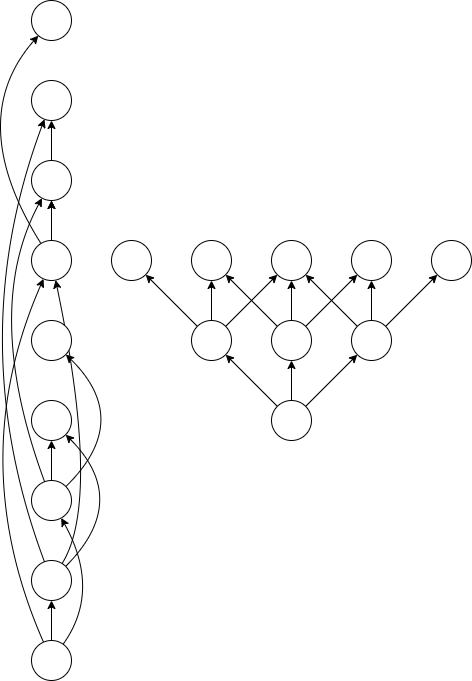
\includegraphics[scale=0.5]{6_3_10_dag.drawio.png}
\end{center}
\newpage
\begin{algorithmic}
  \State $s$ starting node
  \State $path(s)=s$ path vector starting at node s
  \State $G(E,V),(u,v)\in{E}$
  \ForAll{$i=1:n$}
  \State $path(u)+=min(danger(u_i))$
  \EndFor
\end{algorithmic}
*not my best effort, want to finish before class though!
\subsection*{Solution}
\begin{algorithmic}
  \State $D(i,j)$=minimum danger value required to get to block $(i,j)$.
  \State $D(i,j)=min\{D(i-1,j),D(i-1,j-1),D(i-1,j+1)\}+d_{i,j}$
\end{algorithmic}
\end{document}